\chapter{Rastros Temporais da Campanha de Coexistência}
\label{ap:traces}

Os gráficos apresentam exemplos da evolução temporal da janela de congestionamento e do RTT dos oito fluxos simultâneos. Eles complementam a análise agregada do Capítulo~\ref{cap:resultados}, permitindo observar a dinâmica das conexões durante as execuções.

\section{Atraso de gargalo de 10 ms}

\begin{figure}[p]
\centering
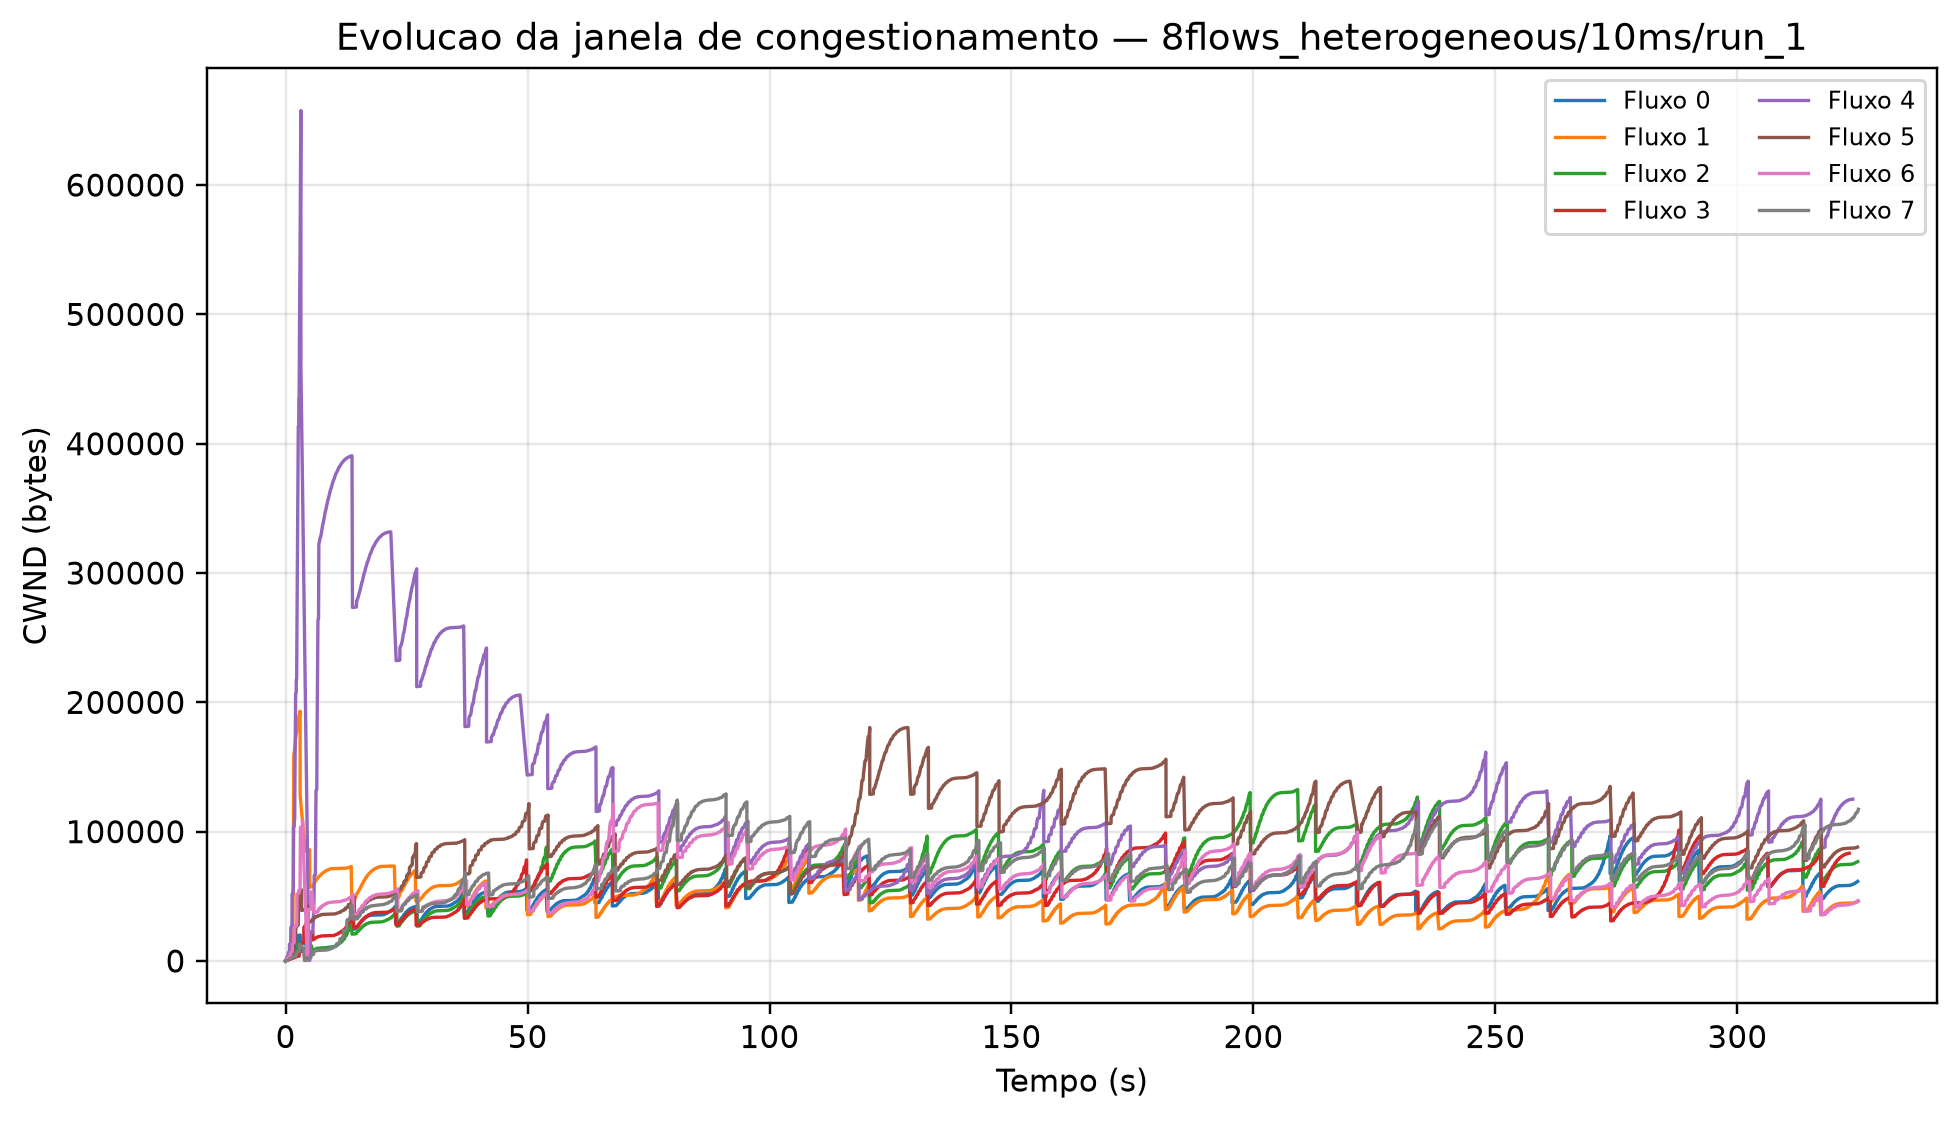
\includegraphics[width=\textwidth]{8flows_heterogeneous_10ms_run_1_cwnd.png}
\caption{Evolução da janela de congestionamento dos oito fluxos, com gargalo de 10 ms.}
\label{fig:trace-cwnd-10}
\end{figure}

\begin{figure}[p]
\centering
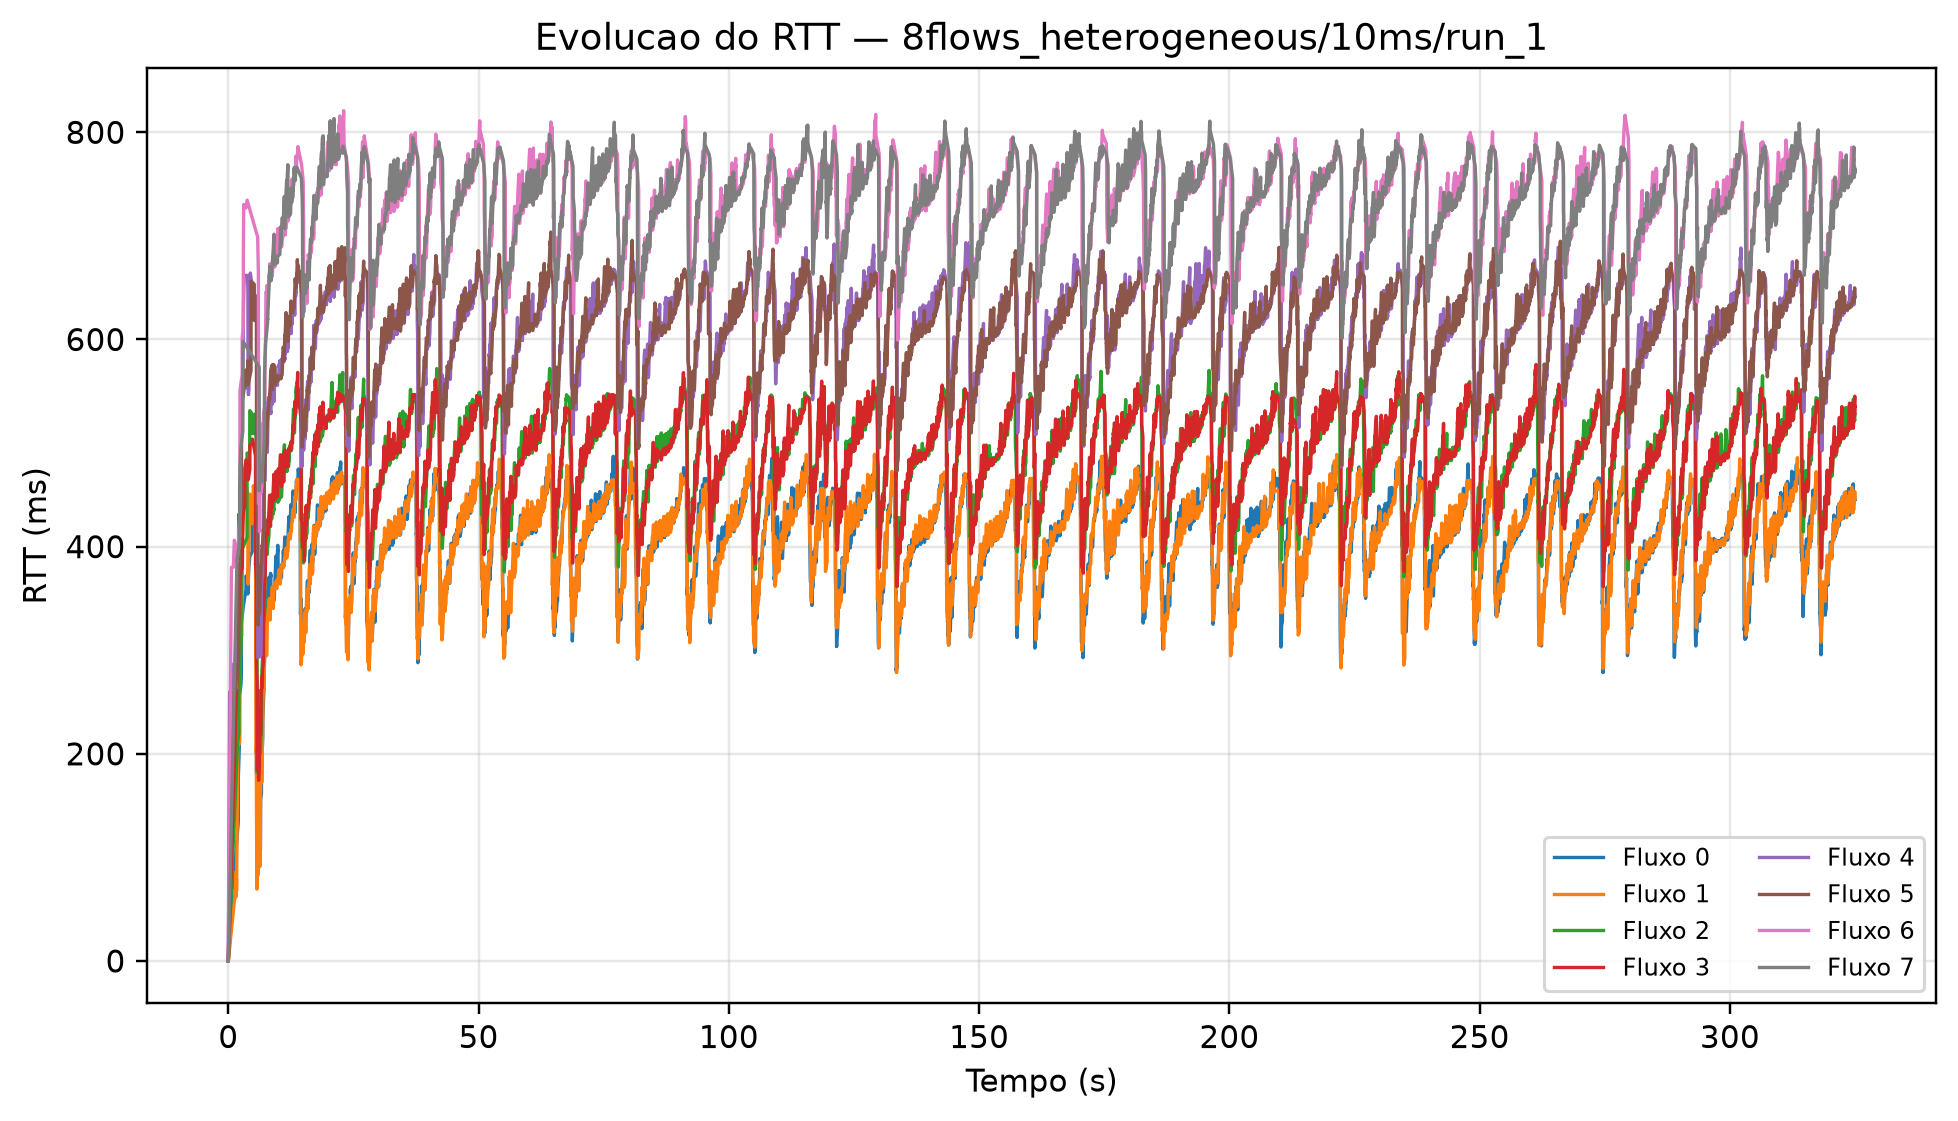
\includegraphics[width=\textwidth]{8flows_heterogeneous_10ms_run_1_rtt.png}
\caption{Evolução do RTT dos oito fluxos, com gargalo de 10 ms.}
\label{fig:trace-rtt-10}
\end{figure}

\section{Atraso de gargalo de 50 ms}

\begin{figure}[p]
\centering
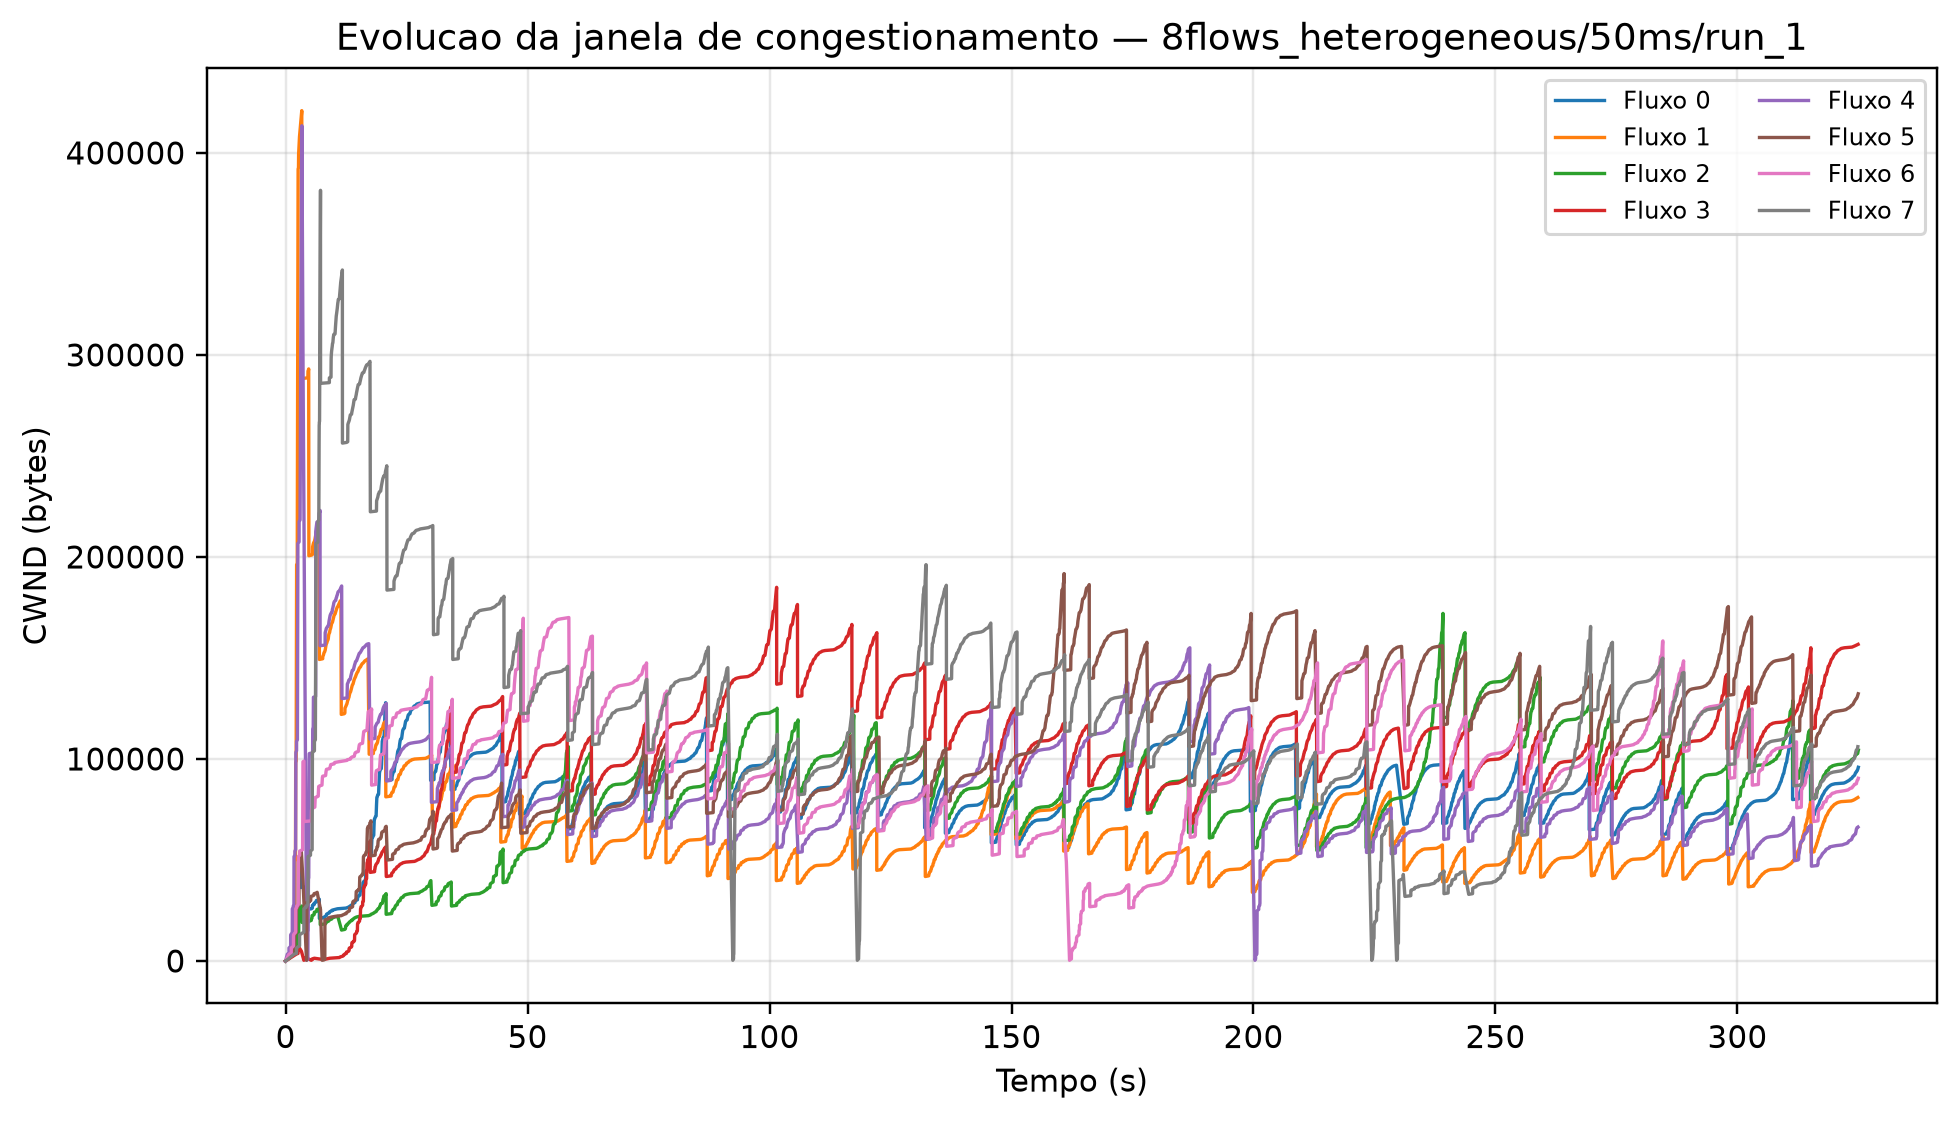
\includegraphics[width=\textwidth]{8flows_heterogeneous_50ms_run_1_cwnd.png}
\caption{Evolução da janela de congestionamento dos oito fluxos, com gargalo de 50 ms.}
\label{fig:trace-cwnd-50}
\end{figure}

\begin{figure}[p]
\centering
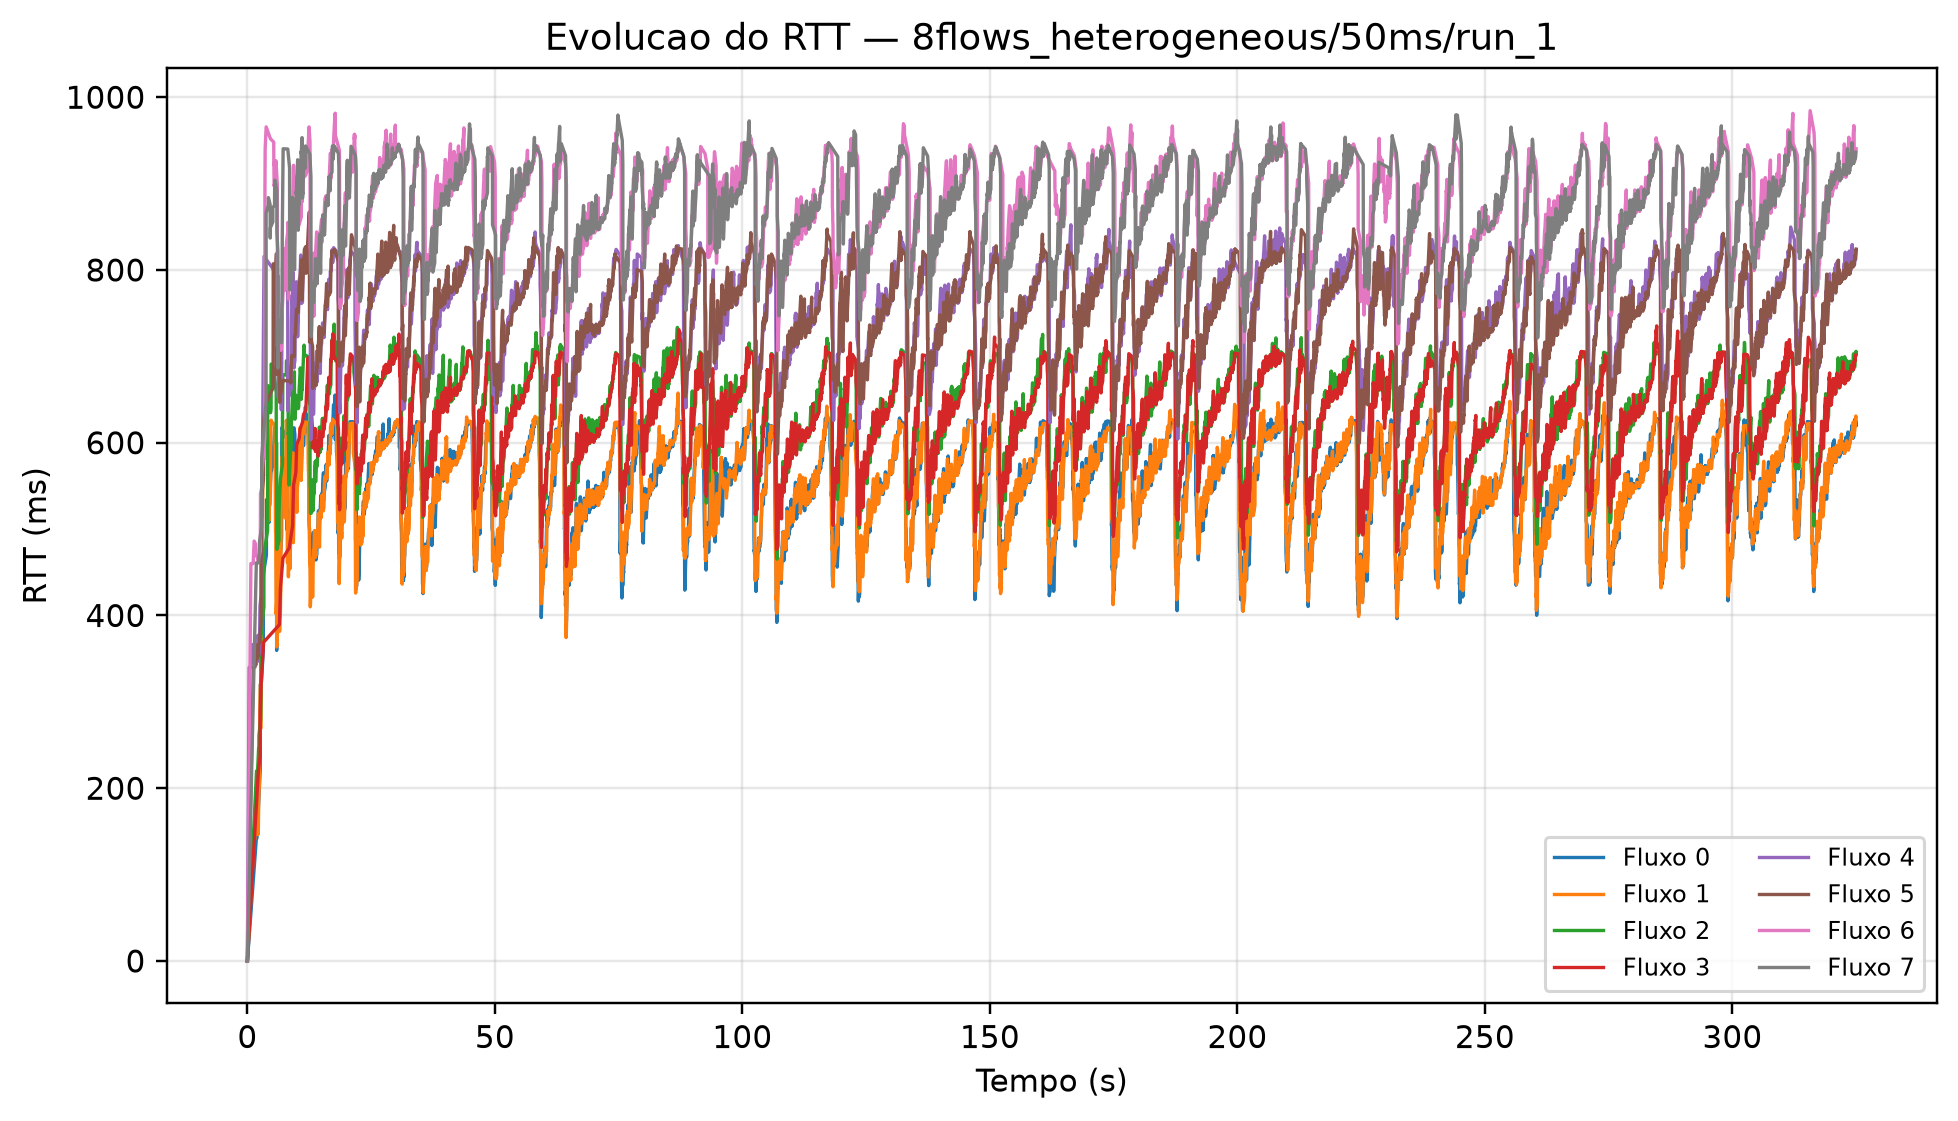
\includegraphics[width=\textwidth]{8flows_heterogeneous_50ms_run_1_rtt.png}
\caption{Evolução do RTT dos oito fluxos, com gargalo de 50 ms.}
\label{fig:trace-rtt-50}
\end{figure}

\section{Atraso de gargalo de 100 ms}

\begin{figure}[p]
\centering
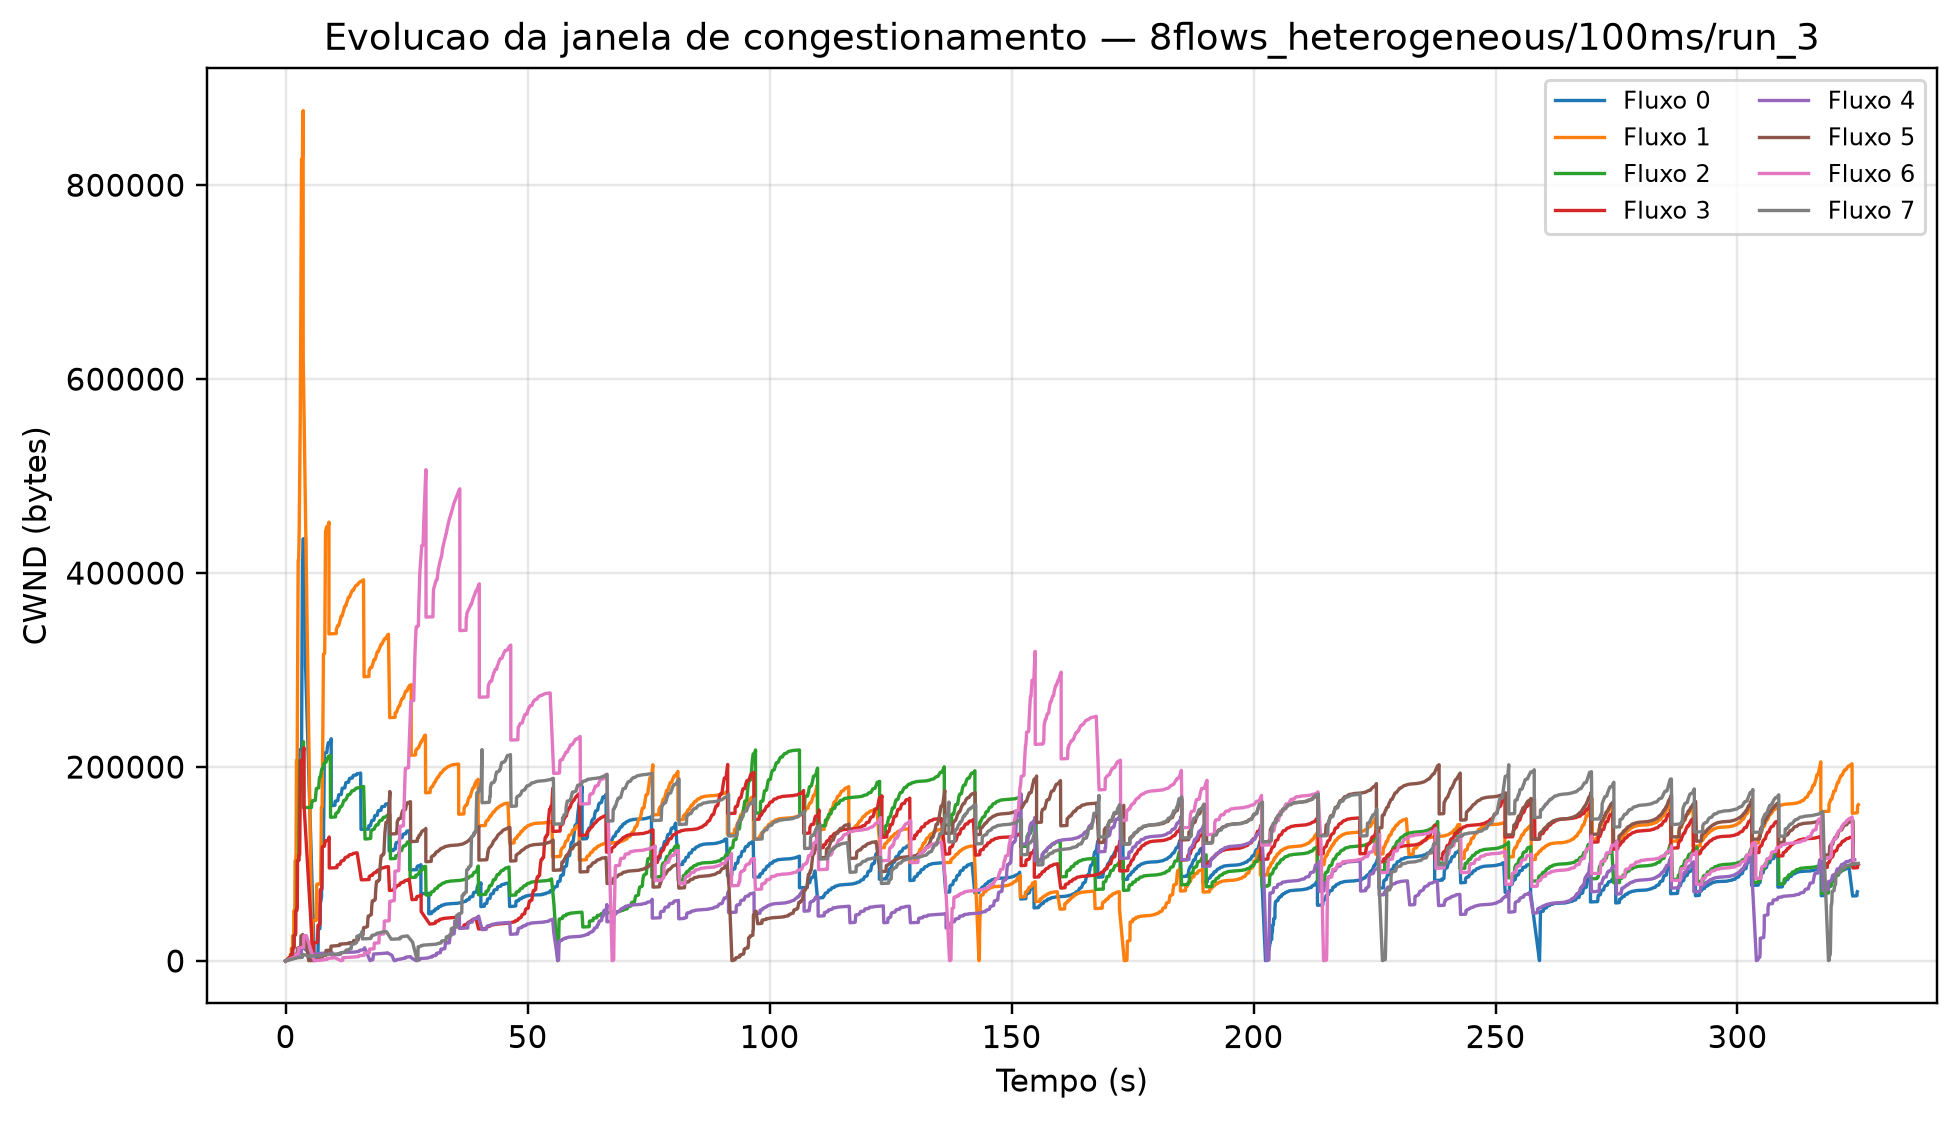
\includegraphics[width=\textwidth]{8flows_heterogeneous_100ms_run_3_cwnd.png}
\caption{Evolução da janela de congestionamento dos oito fluxos, com gargalo de 100 ms.}
\label{fig:trace-cwnd-100}
\end{figure}

\begin{figure}[p]
\centering
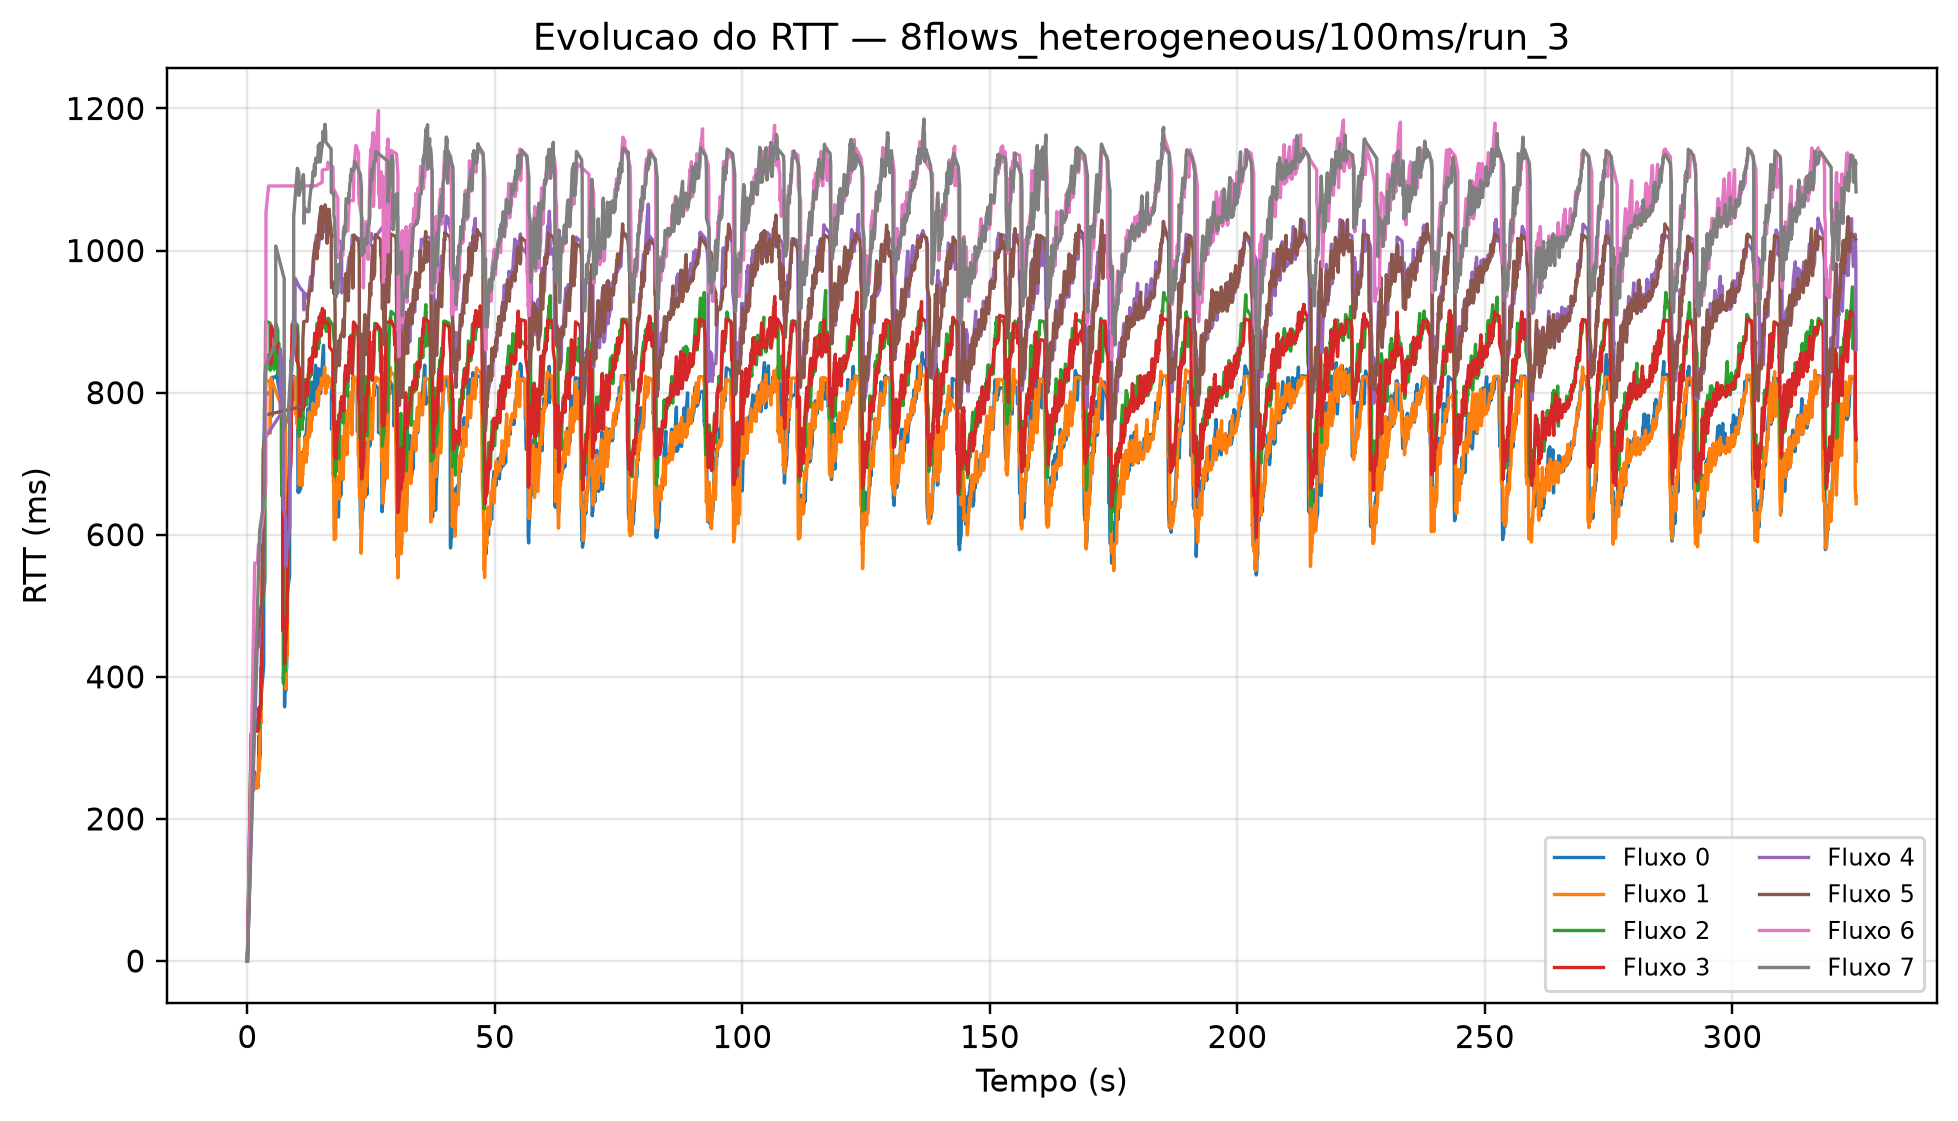
\includegraphics[width=\textwidth]{8flows_heterogeneous_100ms_run_3_rtt.png}
\caption{Evolução do RTT dos oito fluxos, com gargalo de 100 ms.}
\label{fig:trace-rtt-100}
\end{figure}

% --- Referências (ordem alfabética, estilo ABNT) ---
